\section{Experiment 8G: blind end-to-end confirmation}
\label{sec:experiment8g}

\paragraph{Question and frozen predictions.}
Experiment 8G prevents the operating map in Experiment 8F from serving as both
discovery and confirmation. On ten new fleet seeds (106--115), it tests two
points chosen before execution. The primary prediction is that control-aware DP
is viable and isotropic DP is not at $n=20,\epsilon=8$. The secondary prediction
is that both are viable at $n=50,\epsilon=4$. Viability retains the 10\%
tracking-cost limit, full nonlinear amplitude feasibility, and frozen radius
below one. The primary gate additionally requires control-aware improvement in
all ten fleet seeds.

Each test fleet is separate from its training fleet. The comparison includes a
three-second Local fit for every test vehicle, the non-private compatible-family
aggregate, isotropic client-level DP, and control-aware client-level DP. Ten
privacy draws use common random numbers. Local superiority is neither required
nor claimed; its inclusion makes the collaboration tradeoff explicit.

\begin{table}[htbp]
\centering
\caption{Blind Experiment 8G results. Tracking cost is relative to the matching
non-private family aggregate.}
\label{tab:experiment8g}
\begin{tabular}{lrrr}
\toprule
Method & $n=20,\epsilon=8$ & $n=50,\epsilon=4$ & Feasible\\
\midrule
Local & $-11.90$\% & $-11.32$\% & yes\\
Family non-private & 0.00\% & 0.00\% & yes\\
Isotropic DP & 14.40\% & 5.08\% & yes\\
Control-aware DP & 10.43\% & 3.48\% & yes\\
\bottomrule
\end{tabular}
\end{table}

\begin{figure}[htbp]
\centering
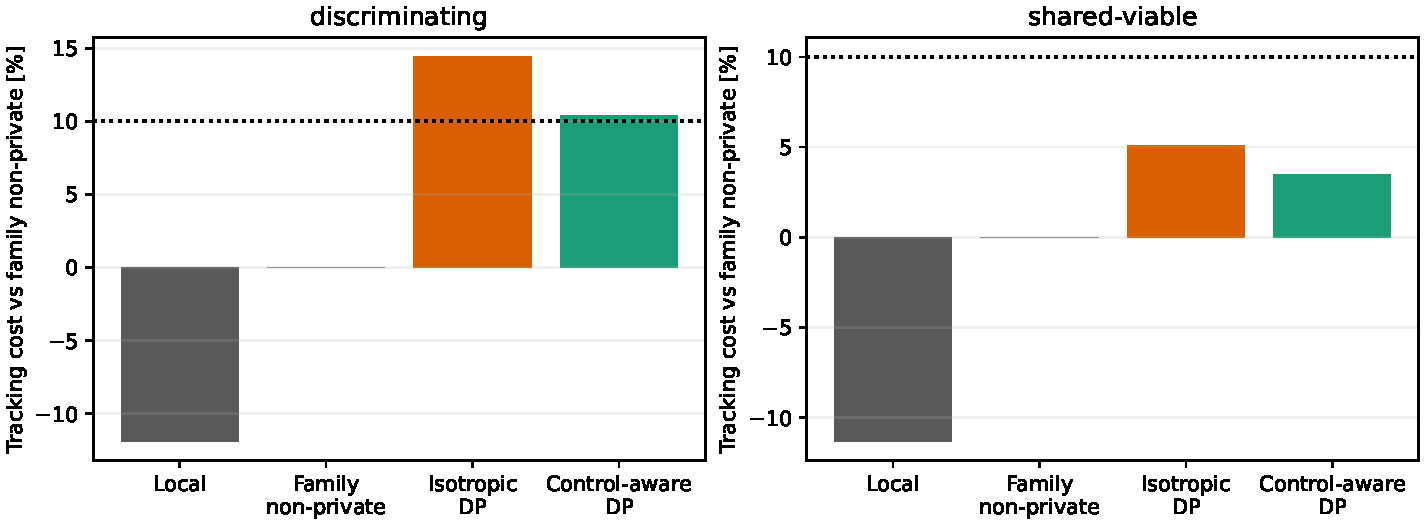
\includegraphics[width=0.9\linewidth]{../results/figures/experiment_8g_blind_confirmation.pdf}
\caption{Blind comparison at the two frozen deployment points. The dotted line
is the unchanged 10\% tracking-cost boundary.}
\label{fig:experiment8g}
\end{figure}

\paragraph{Results.}
All 1,800 local fits converge. The run contains 1,200 private family releases
and 39,600 nonlinear client--scenario evaluations. All methods are
amplitude-feasible and have worst frozen radius below one. At the primary point,
control-aware DP improves on isotropic DP in every fleet seed, with a 3.47\%
mean gain and one-sided paired Wilcoxon $p=0.000977$. Nevertheless, its 10.43\%
cost narrowly exceeds the frozen limit; isotropic DP costs 14.40\%. The primary
confirmation gate therefore fails. At the secondary point, both mechanisms
confirm as viable: control-aware DP costs 3.48\% and isotropic DP 5.08\%.

Local identification has the best absolute tracking and lower mean parameter
error. Its tracking is 11.90\% and 11.32\% better than the respective
non-private family aggregates. This repeats the earlier boundary finding that
federation does not improve a highly efficient Local estimator in this
benchmark; the supported benefits are privacy-preserving shared calibration and
model consolidation.

\paragraph{Decision.}
Experiment 8G is a negative primary gate and a positive secondary confirmation.
The manuscript must not claim that 20 clients suffice at $\epsilon=8$ under a
strict 10\% criterion. Its headline confirmed point is instead
$n=50,\epsilon=4$, while the 20-client outcome defines a close but unsupported
boundary. The all-seed directional improvement supports control-aware shaping,
but does not override the failed absolute-utility criterion. No post-hoc
threshold or weight adjustment is warranted.

\paragraph{Reproducibility.}
The frozen protocol is in \path{code/config/experiment_8g.json}; the runner is
\path{code/experiments/experiment_8g_blind_confirmation.py}. Aggregate,
seed--draw, paired, and conclusion files are stored under \path{results/tables}.
